\documentclass[aspectratio=169,11pt]{beamer}
\usetheme{default}
\usecolortheme{seagull}
\setbeamertemplate{navigation symbols}{}
\setbeamertemplate{footline}[frame number]
\setbeamerfont{frametitle}{size=\large,series=\bfseries}
\setbeamerfont{title}{size=\Large,series=\bfseries}
\usepackage{graphicx}
\graphicspath{{./}{../figures/}}
\newcommand{\src}[1]{\vfill{\tiny\textcolor{gray}{#1}}}

\title{HLA regions from 610 assembled haplotypes: extraction, typing and pangenome views}
\author{Robert Hoehndorf (KAUST)}
\institute{BioHackathon Japan 2026, HLA/pangenome group}
\date{15 September 2026}

\begin{document}

\begin{frame}
  \titlepage
\end{frame}

\begin{frame}{One CWL workflow: pgr-tk extraction, Immuannot typing, pgr-tk and pggb graphs}
  \begin{itemize}
    \item 610 haplotypes: APR (UAE Arab) 106, HPRC release 2 464, JaSaPaGe Saudi 18 and Japanese 20, GRCh38, CHM13
    \item MHC (GRCh38 chr6:28.5--33.5 Mb, 100 kb flank) pulled from each assembly with pgr-tk \texttt{pgr-query}, about 30 s per genome
    \item Immuannot (IPD-IMGT/HLA 3.55) gives gene structure and full-resolution allele calls per haplotype
    \item Per gene (19 genes): sequences cut at the Immuannot coordinates, pgr-tk principal-bundle plots, pggb graphs rendered with odgi
    \item Whole MHC and the class II block (DRA to DMA): pgr-tk bundle decomposition, dendrograms, bundle graphs
    \item Runs on the NIG node without containers (Toil, \texttt{--no-container}); repo \texttt{github.com/leechuck/pangenome-bh26}
  \end{itemize}
\end{frame}

\begin{frame}{The MHC comes out intact from 608 of 610 haplotypes}
  \centering
  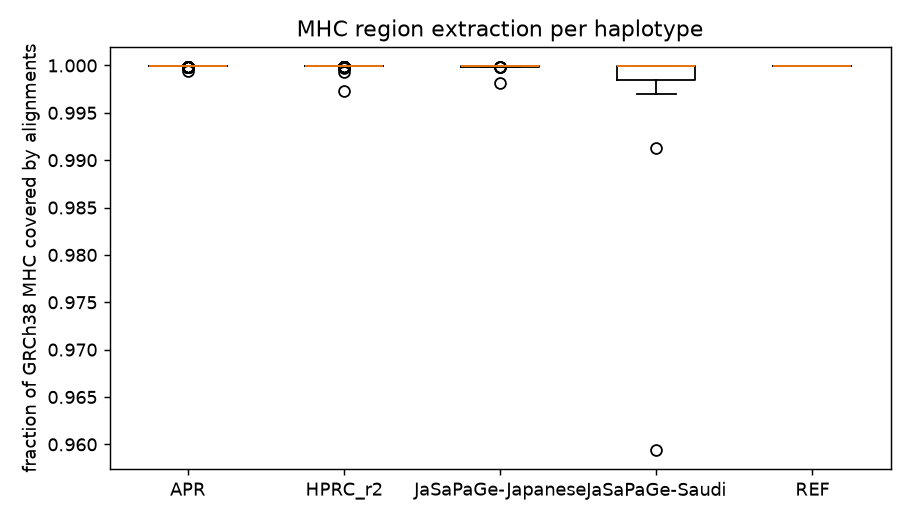
\includegraphics[height=0.62\textheight]{mhc_extraction_coverage.png}
  \begin{itemize}
    \item y: fraction of the GRCh38 MHC covered by the extracted segments; median 1.000 in every cohort, 599 haplotypes on a single contig
    \item Five 1000G JPT individuals were assembled by both HPRC and JaSaPaGe: 59 of 61 full-resolution gene calls agree, the two exceptions differ only in an intron
  \end{itemize}
\end{frame}

\begin{frame}{Allele frequencies separate the cohorts; DRB1 full-length sequences are mostly new}
  \centering
  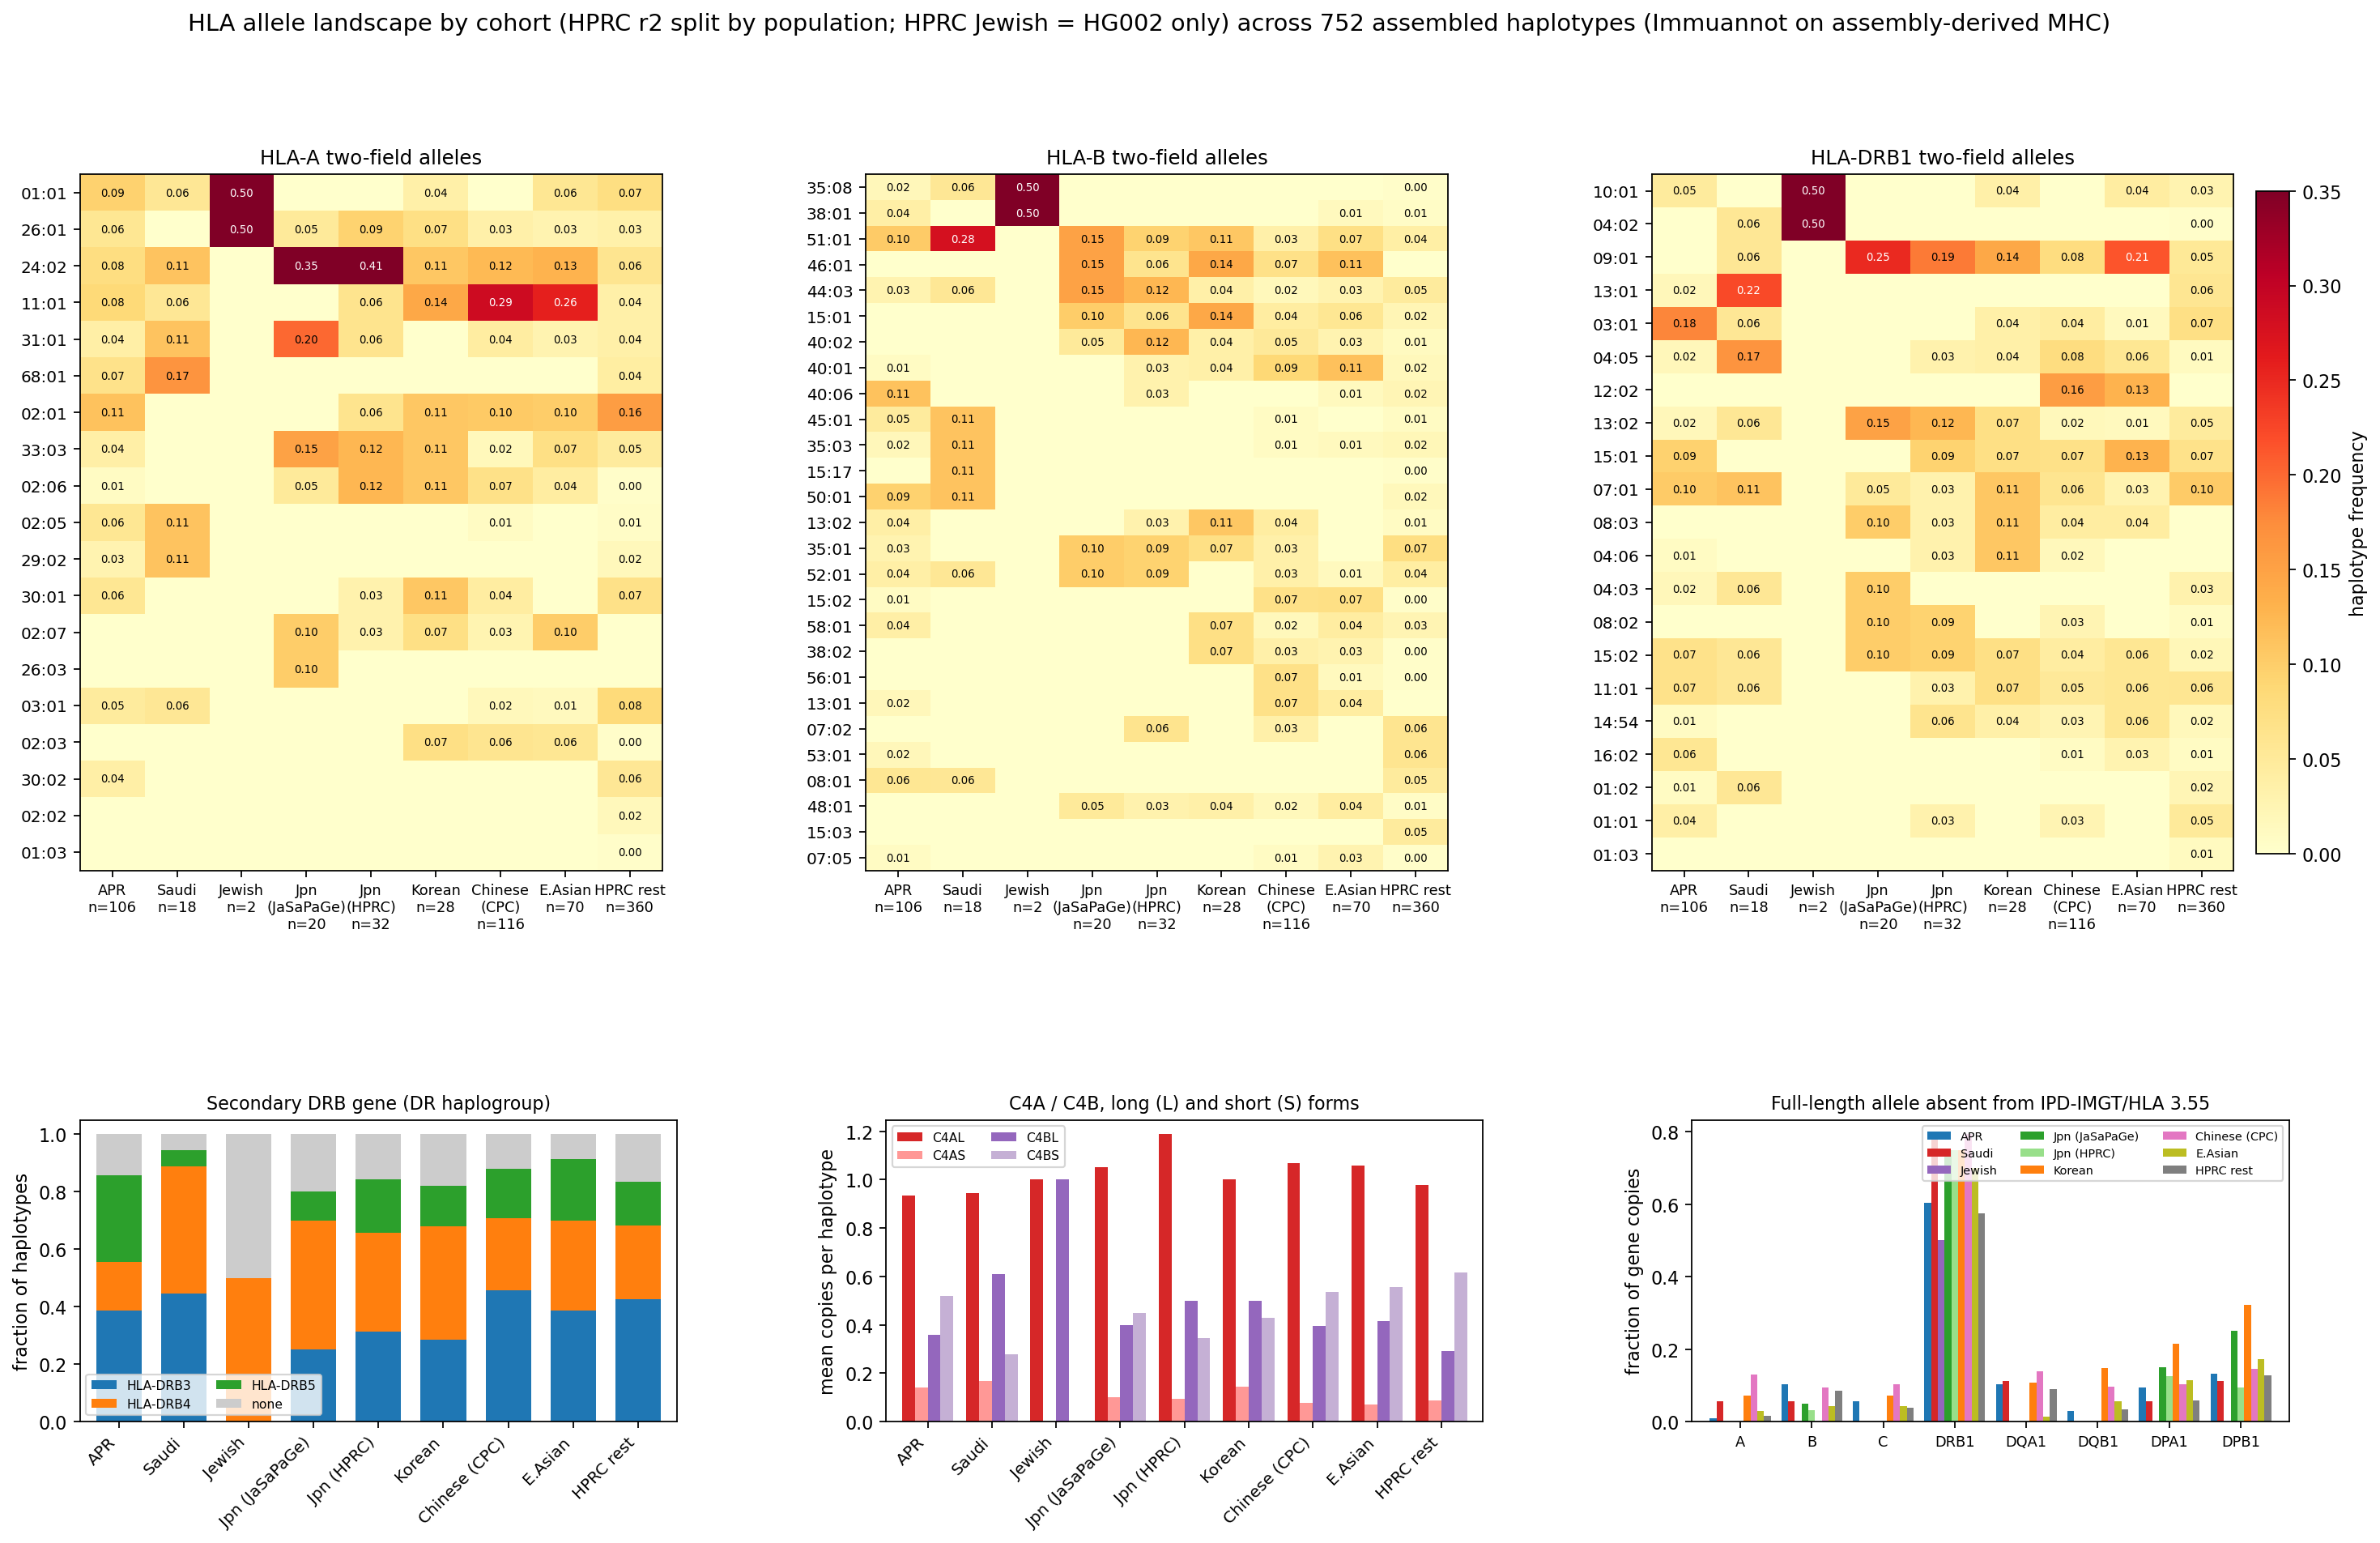
\includegraphics[height=0.78\textheight]{fig5_population_hla.png}
  \src{Immuannot consensus calls, two-field alleles; novel = full-length sequence absent from IPD-IMGT/HLA 3.55}
\end{frame}

\begin{frame}{Two HPRC individuals are truly MHC-homozygous; one JaSaPaGe assembly carries the same haplotype twice}
  \centering
  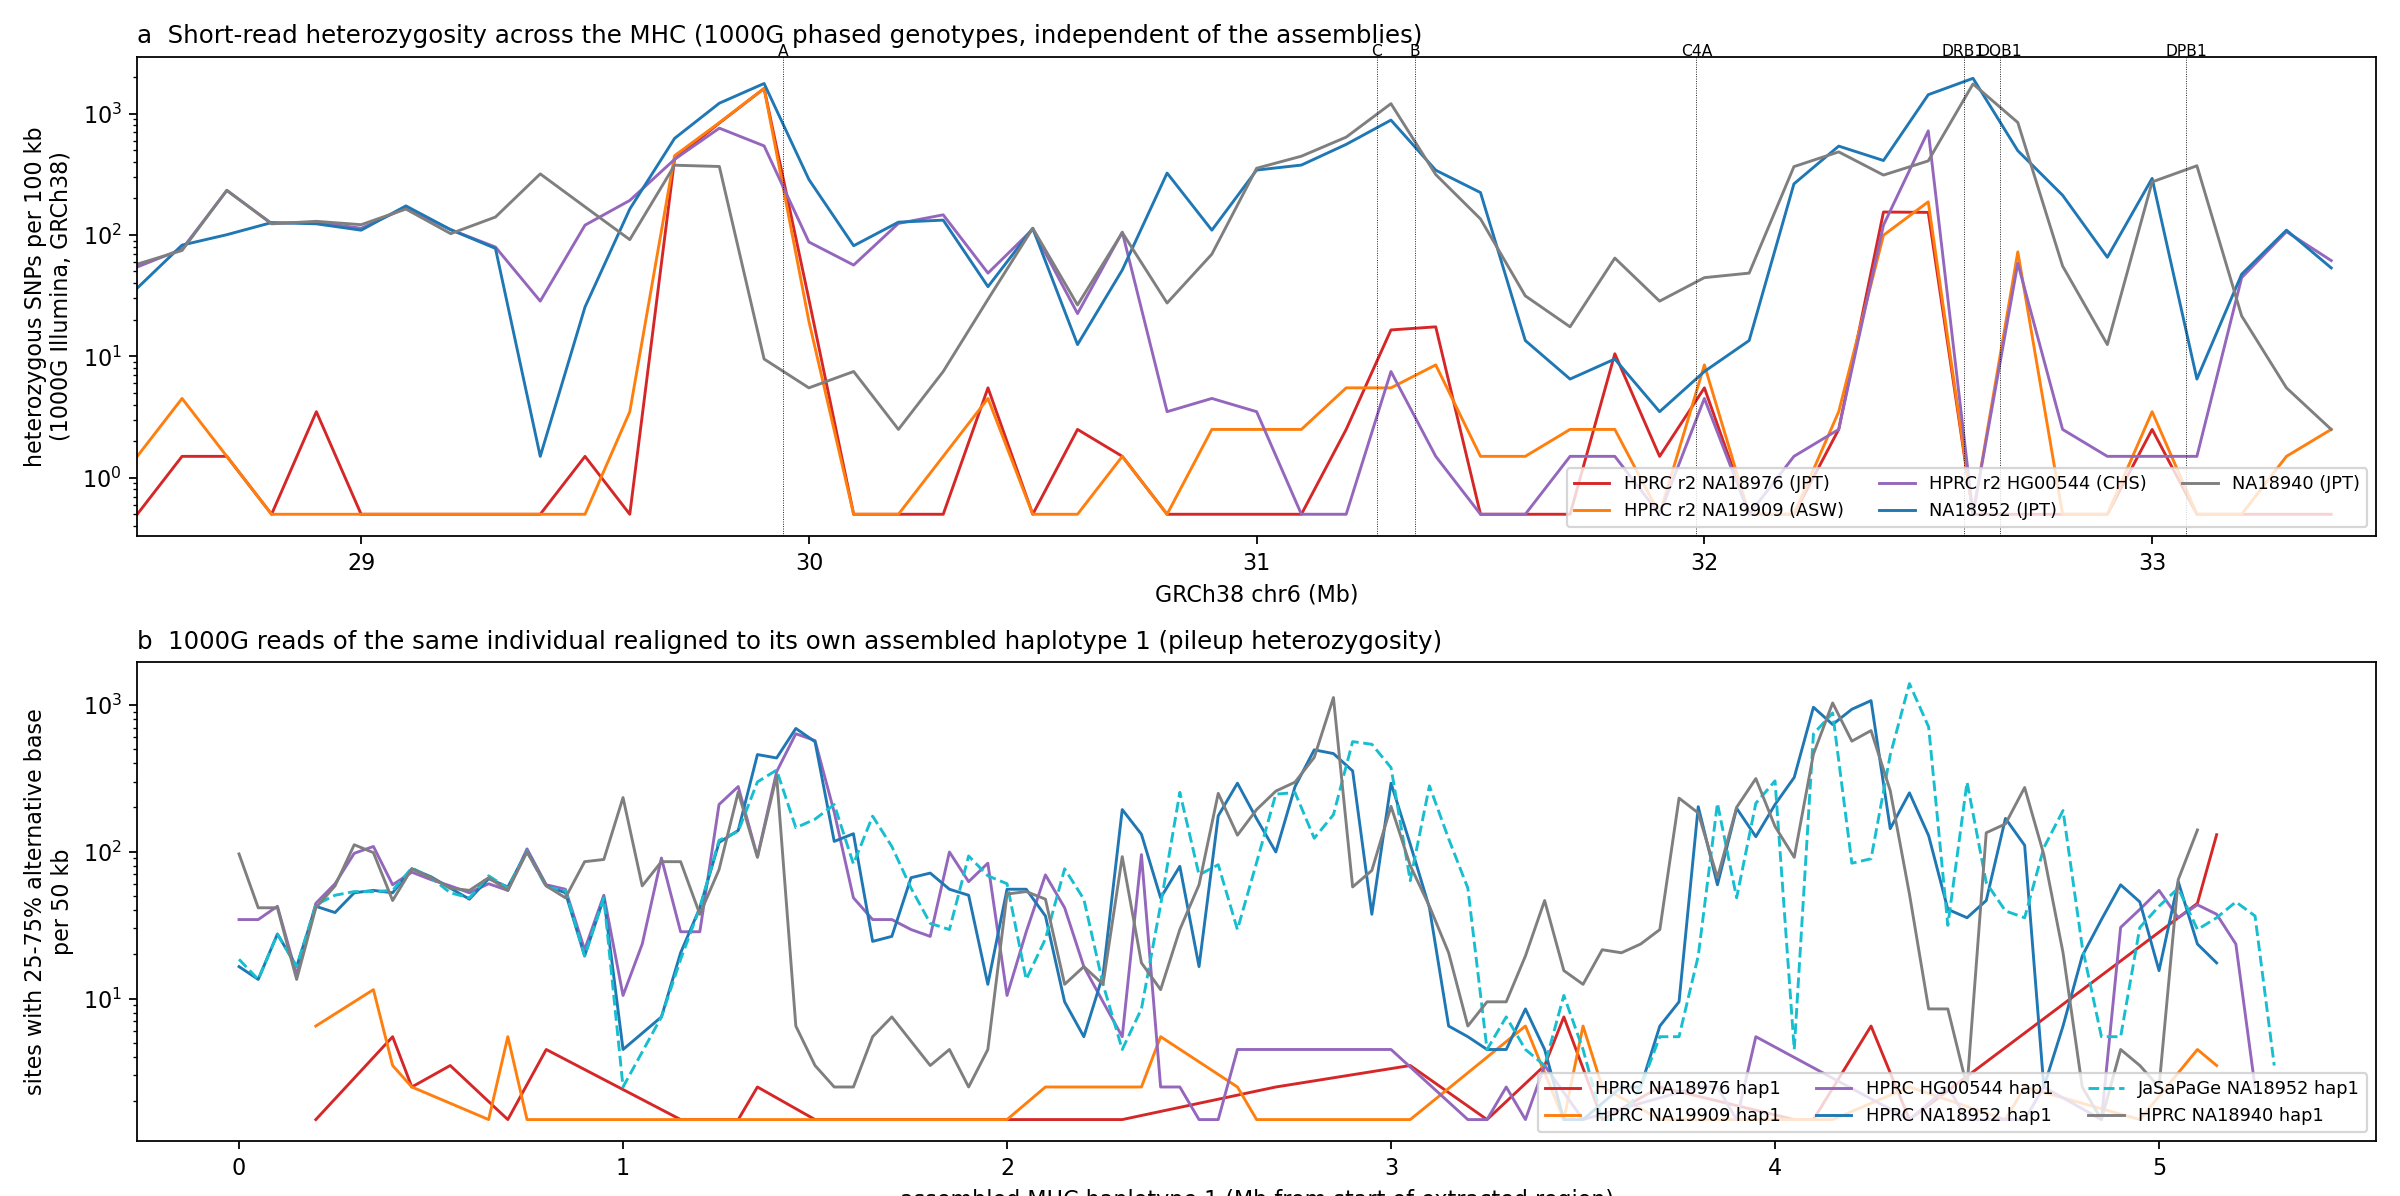
\includegraphics[width=0.8\textwidth]{fig3_ab.png}
  \begin{itemize}
    \item NA18976, NA19909 (red, orange): under 100 heterozygous 1000G SNPs across 5 Mb, matching their two near-identical assembled haplotypes; JaSaPaGe NA18952 (dashed): own reads show full heterozygosity on both ``haplotypes'', hap1 = hap2
  \end{itemize}
\end{frame}

\begin{frame}{Substitution-type novel coding alleles hold up in the individual's own reads; indel-only ones do not}
  \centering
  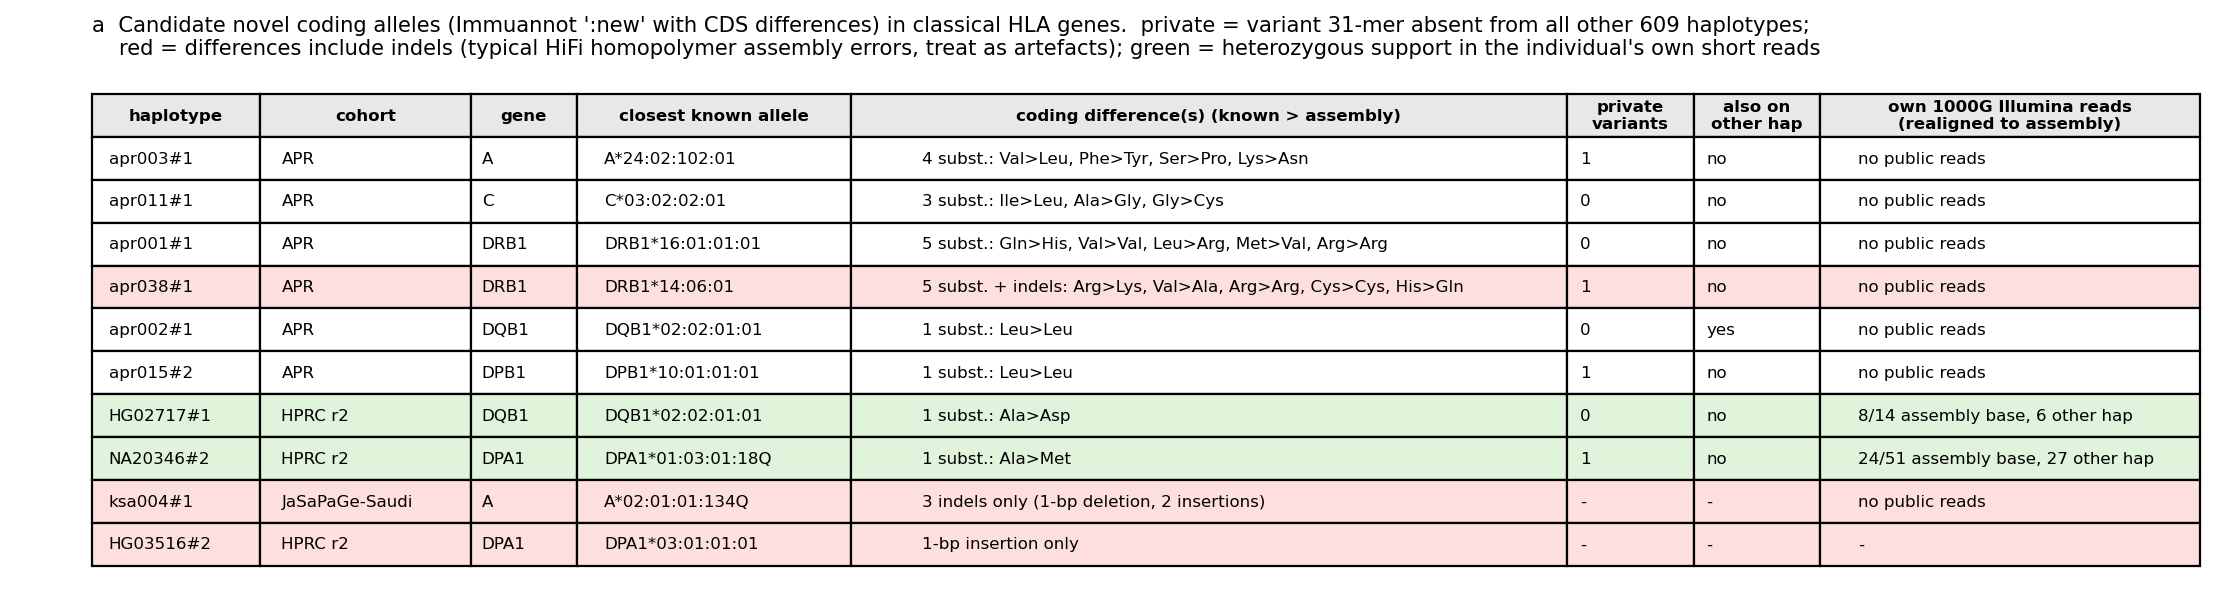
\includegraphics[width=0.92\textwidth]{fig4_table.png}\\[2pt]
  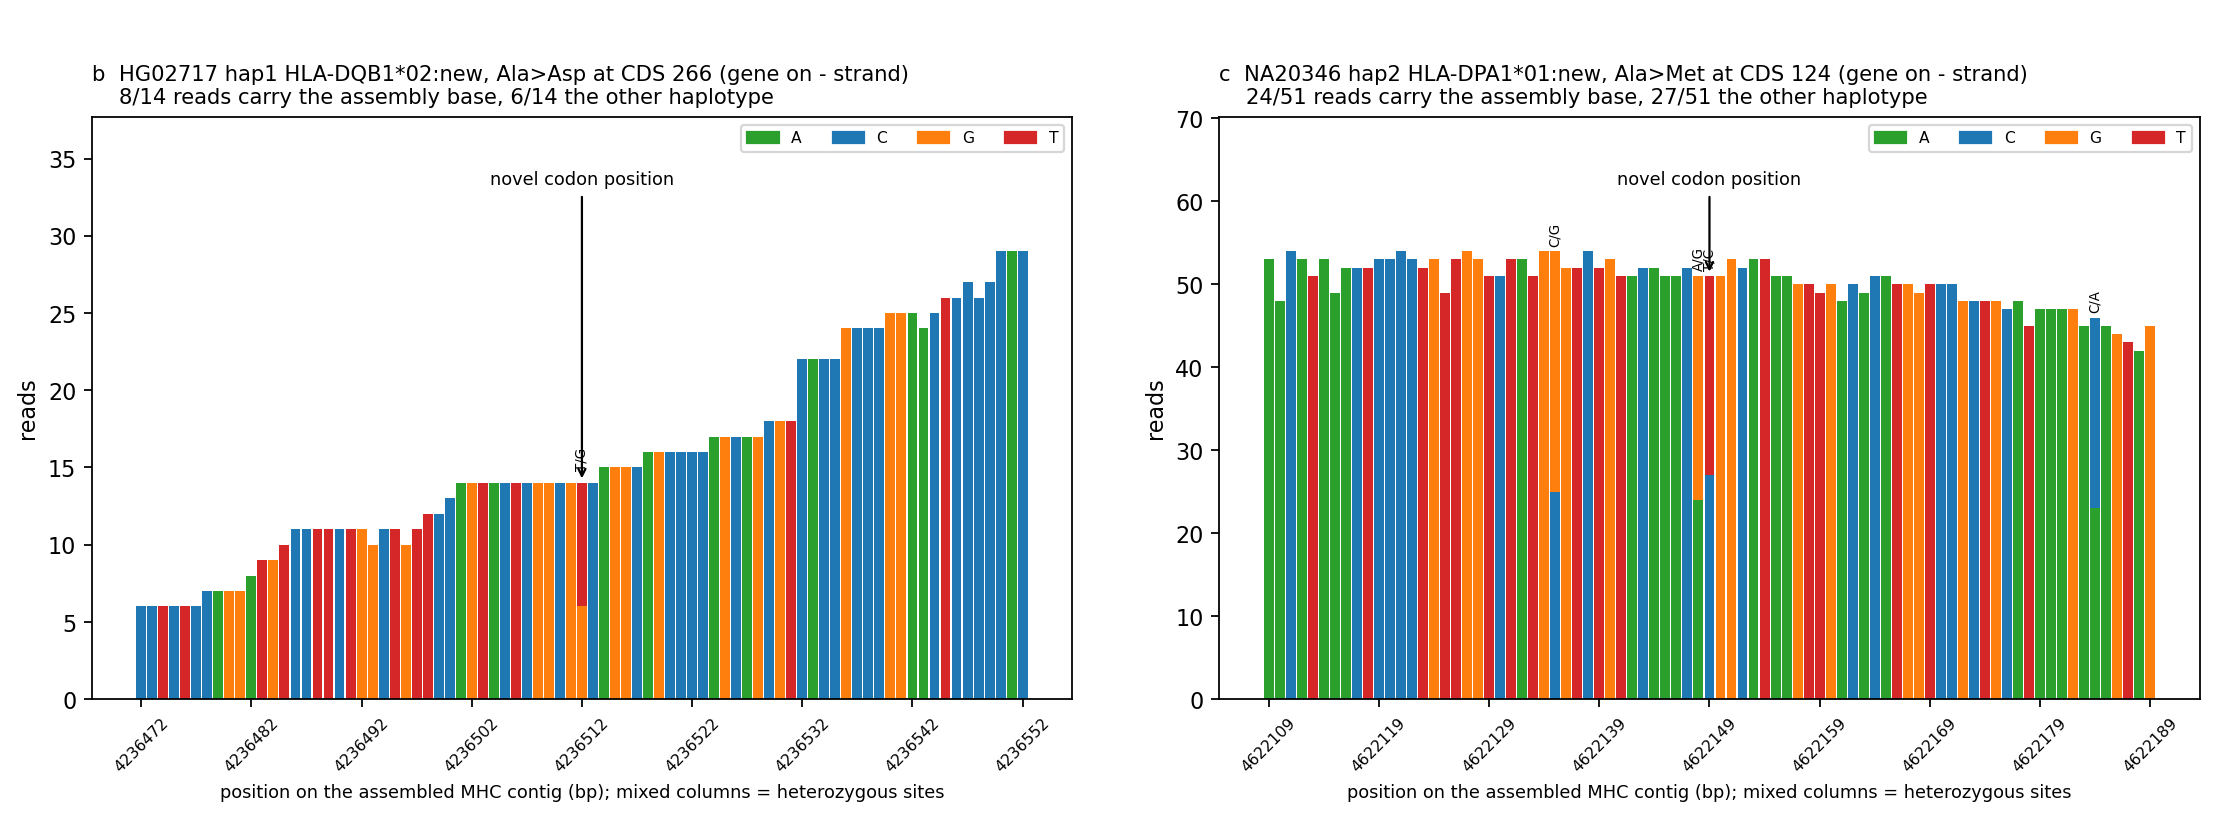
\includegraphics[height=0.3\textheight]{fig4_pileups.png}
  \src{Pileups: the individual's 1000G Illumina reads realigned to its assembled contig; mixed columns = heterozygous sites. APR and JaSaPaGe reads are not public}
\end{frame}

\begin{frame}{425 distinct gene-level class II haplotypes among 608; secondary DRB gene structures the flow}
  \centering
  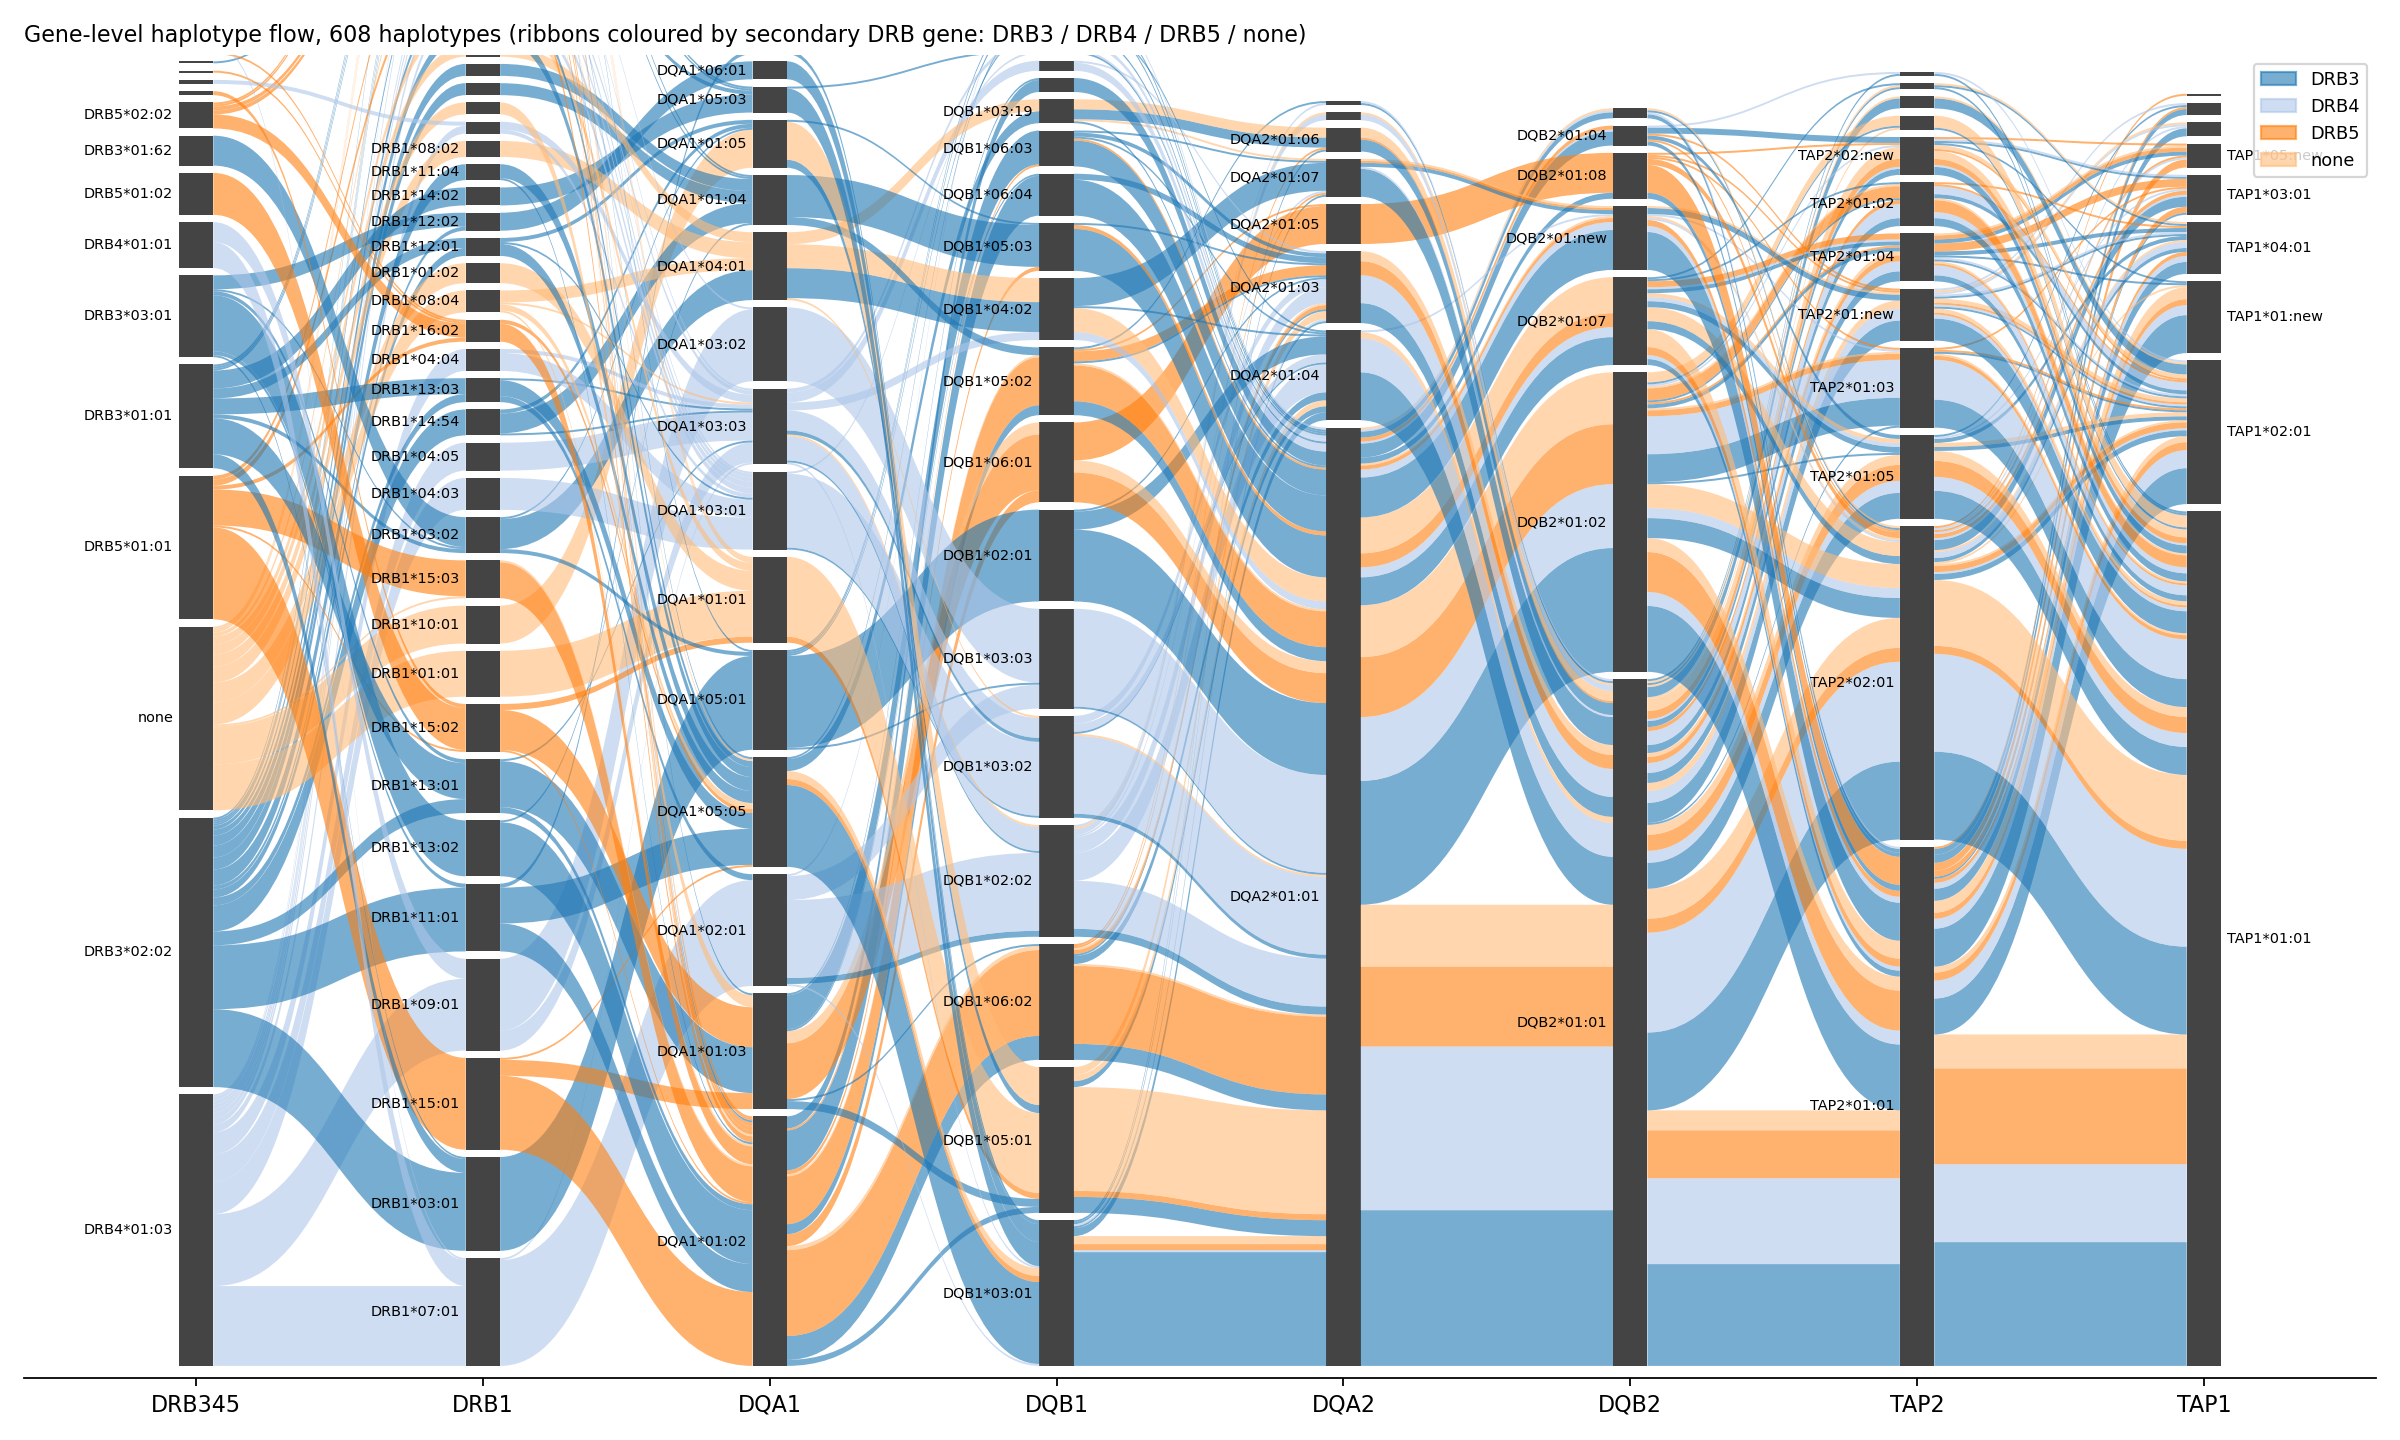
\includegraphics[height=0.78\textheight]{fig6_classII_haplotype_flow.png}
  \src{Two-field alleles per haplotype; ribbons coloured by DRB3 / DRB4 / DRB5 / none. After Chin, ASHI 2023 (94 haplotypes)}
\end{frame}

\begin{frame}{The DR-DQ block differs by population}
  \centering
  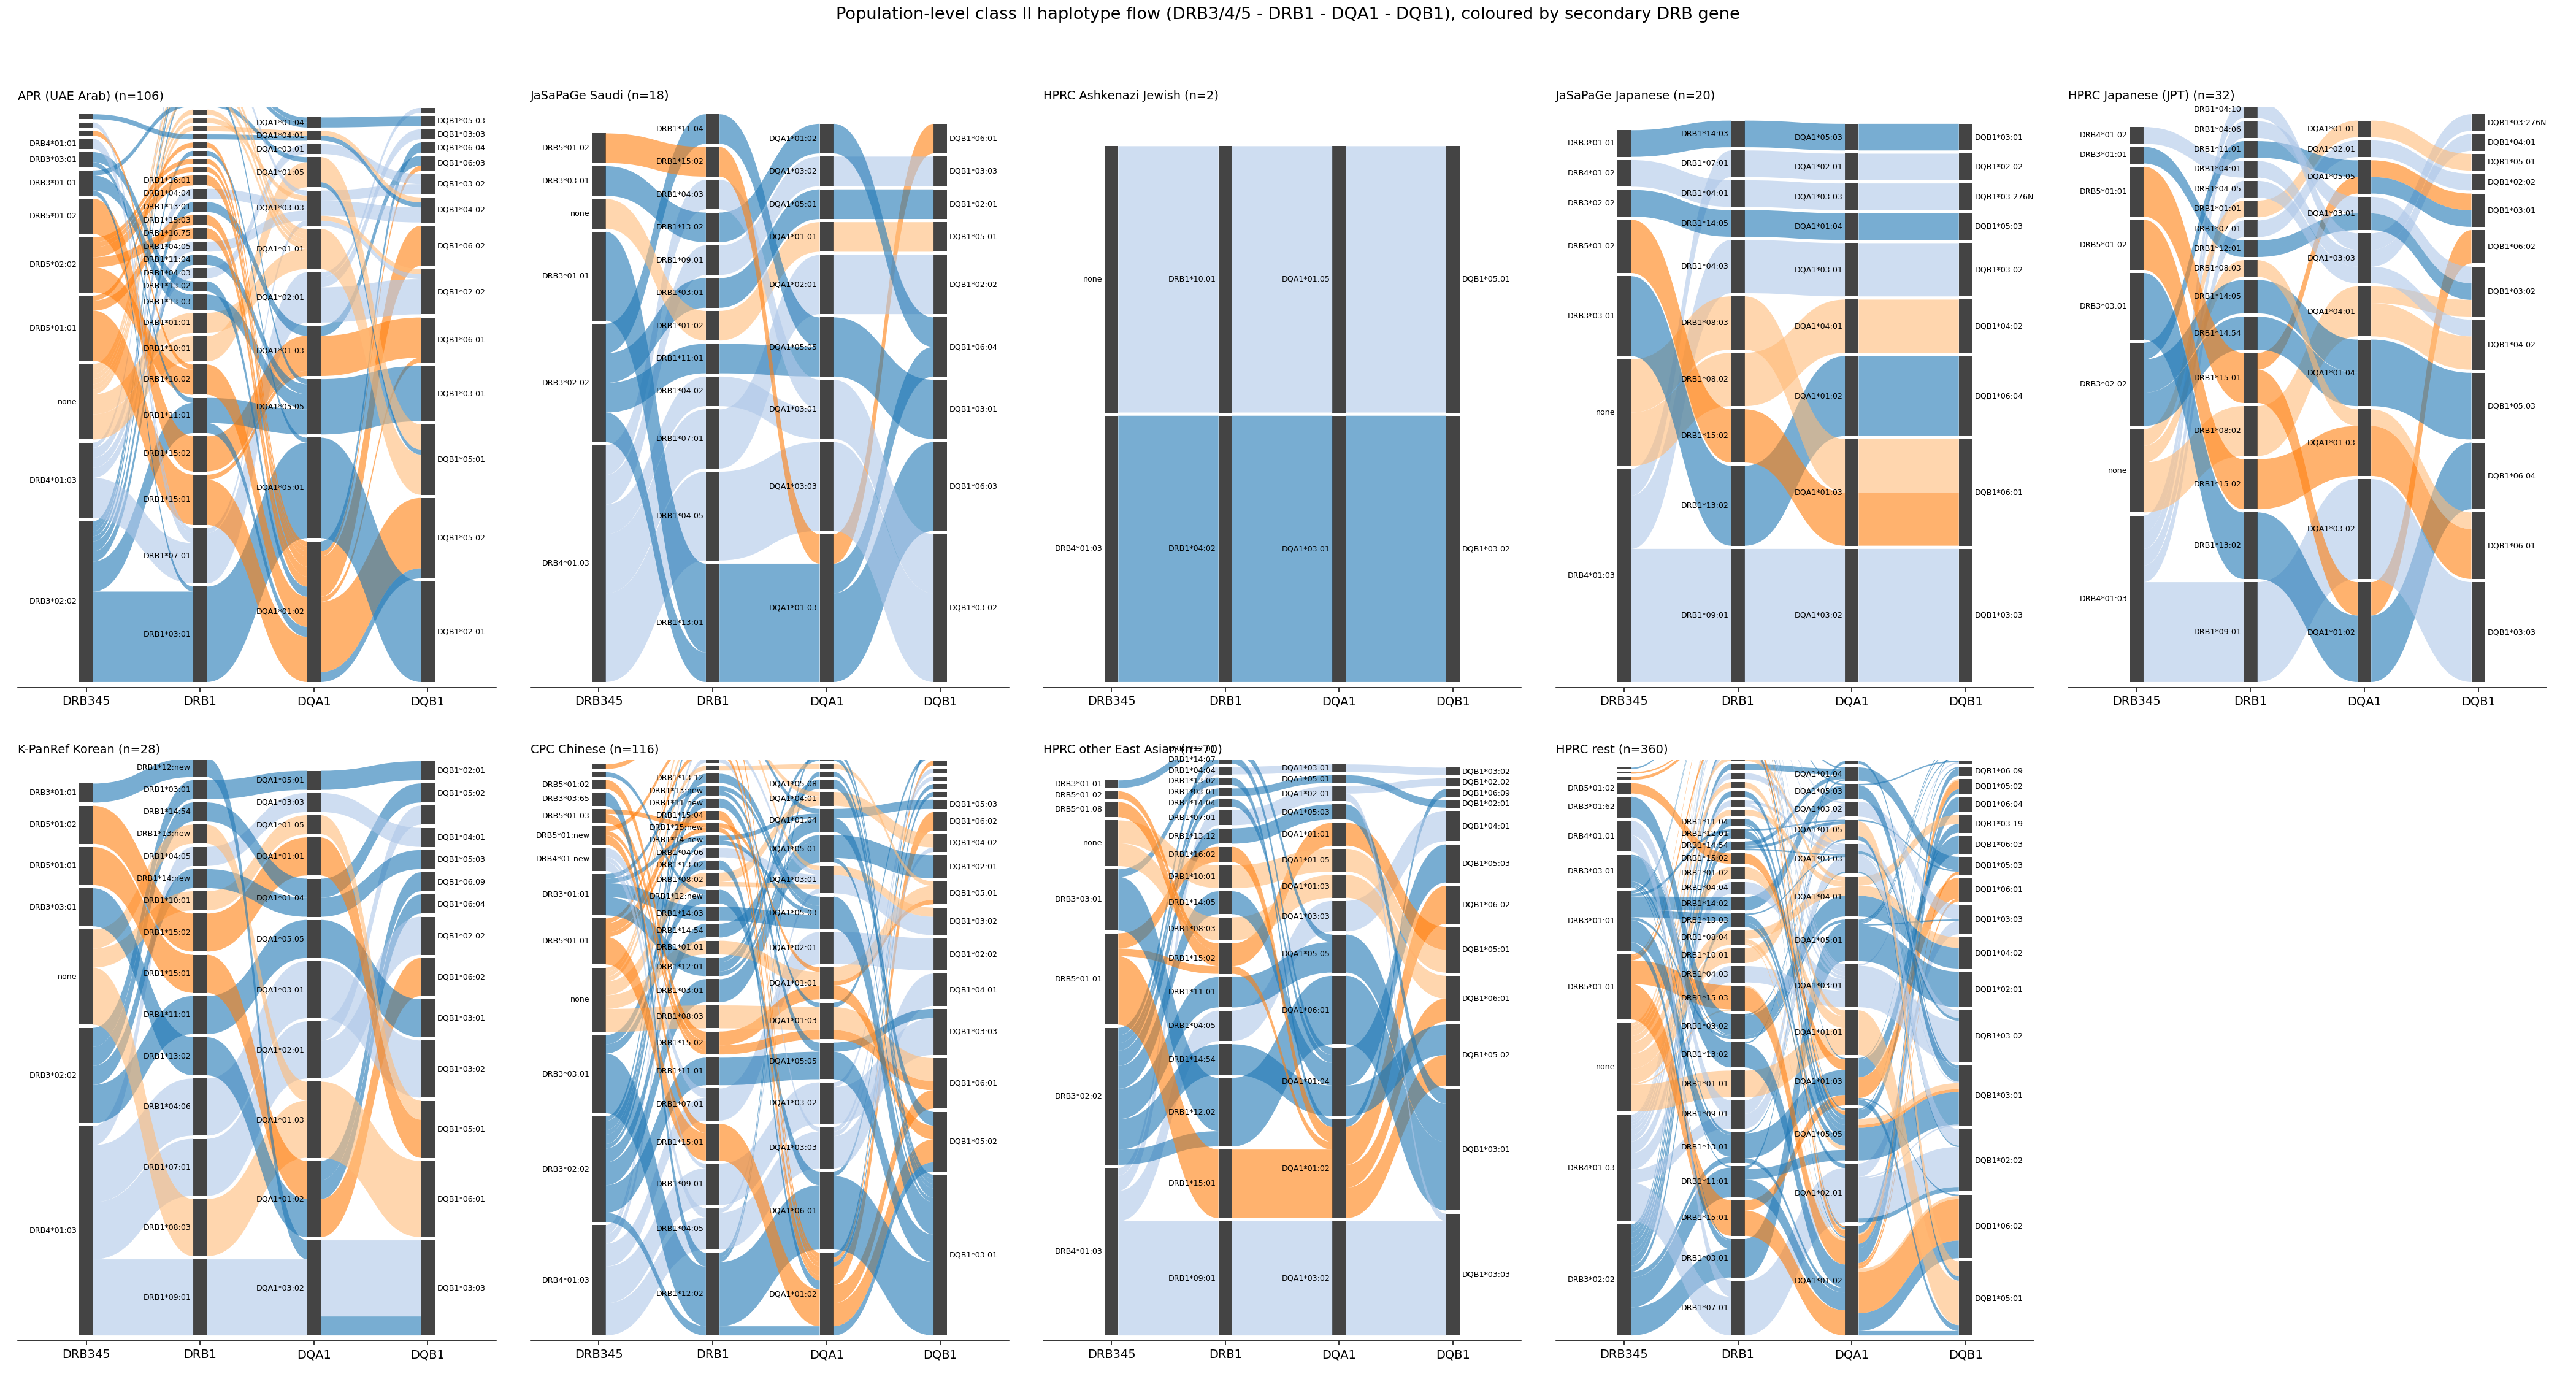
\includegraphics[width=\textwidth]{fig7_classII_flow_by_cohort.png}
  \begin{itemize}
    \item Saudi: DRB4 haplotypes (DR7, DR4) 44\%; Japanese: DRB1*09:01--DQB1*03:03 and DRB1*15:02--DQB1*06:01; APR: DRB1*03:01--DQB1*02:01 18\%
  \end{itemize}
\end{frame}

\begin{frame}{Sequence-level structure of the class II region follows the DR haplogroups}
  \centering
  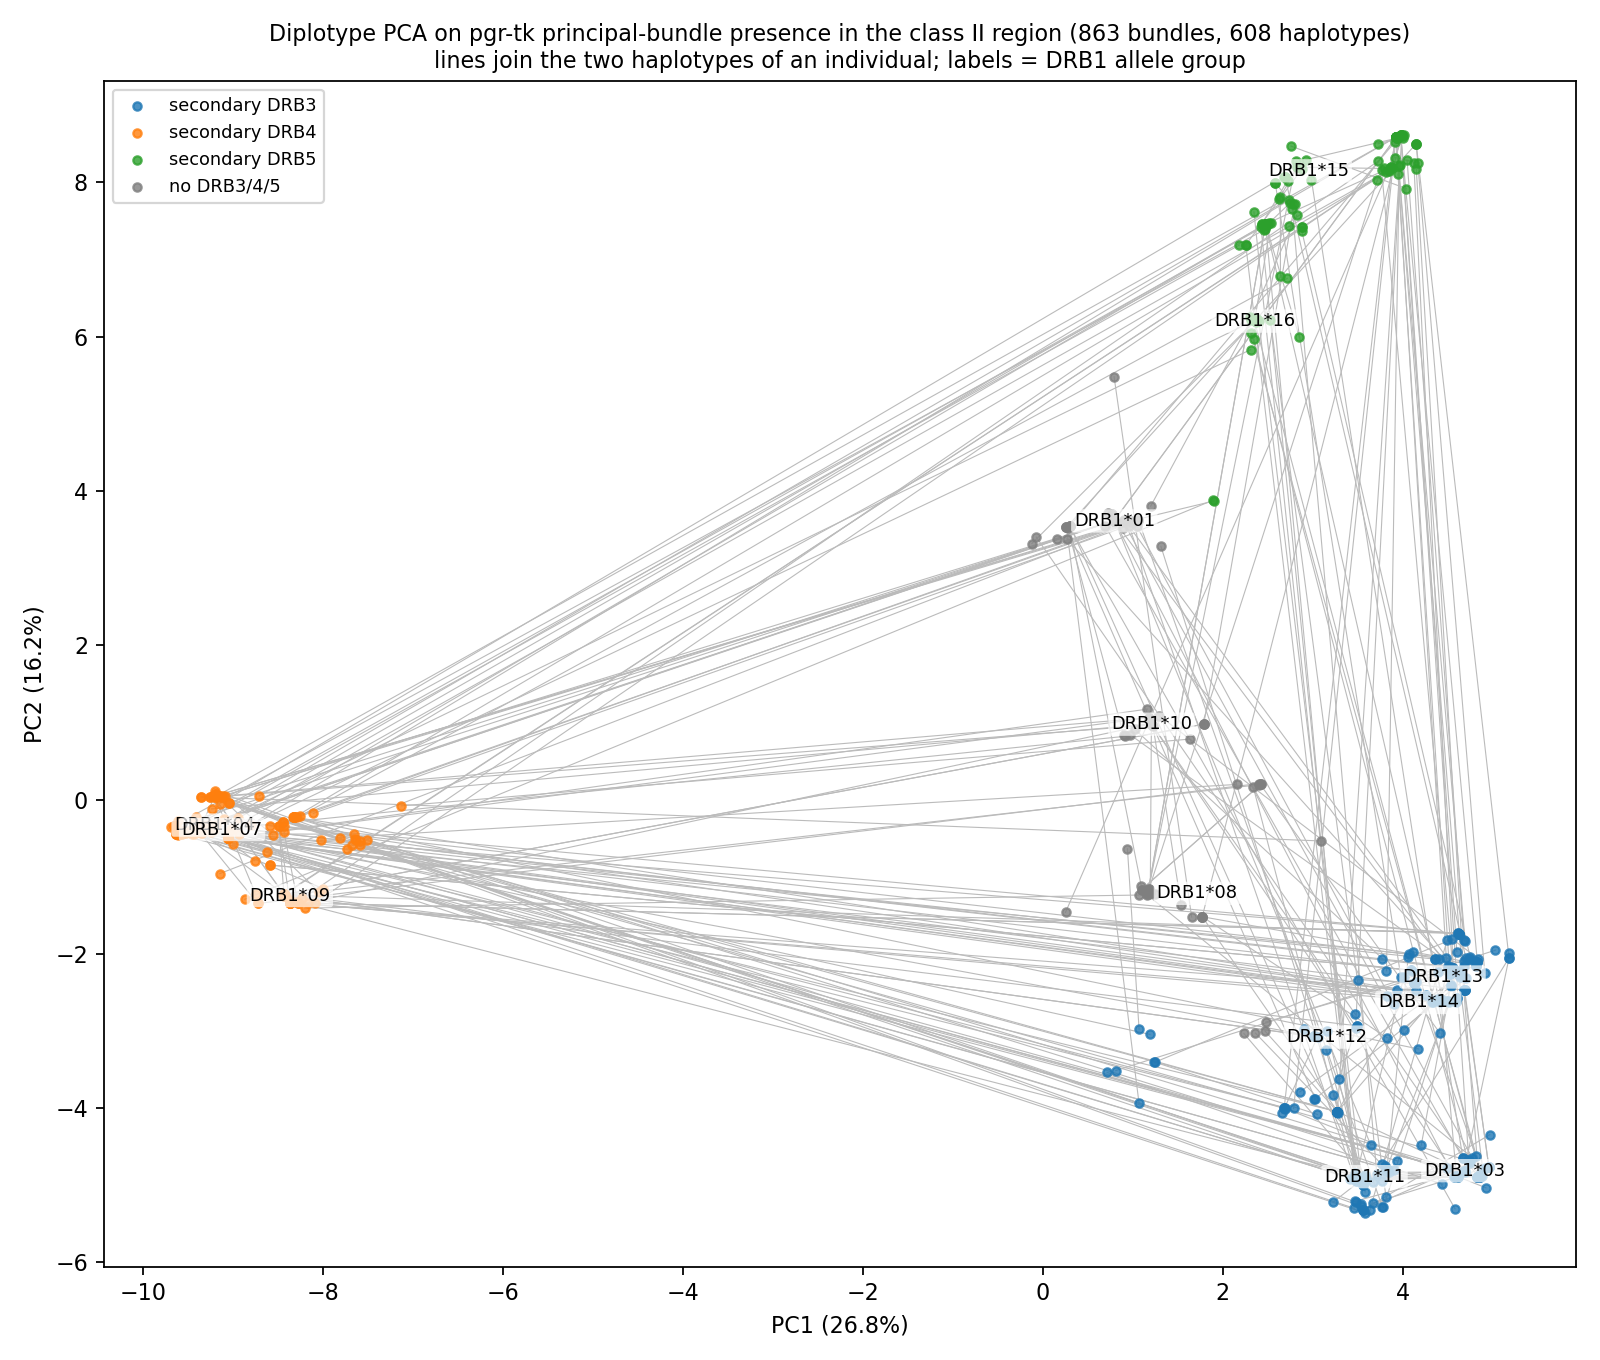
\includegraphics[height=0.78\textheight]{fig11_classII_bundle_pca.png}
  \src{PCA on presence of 863 pgr-tk principal bundles (DRA to DMA); each point one haplotype, grey lines join the two haplotypes of an individual}
\end{frame}

\begin{frame}{Bundle-distance clusters are near-pure DRB1 allele groups}
  \centering
  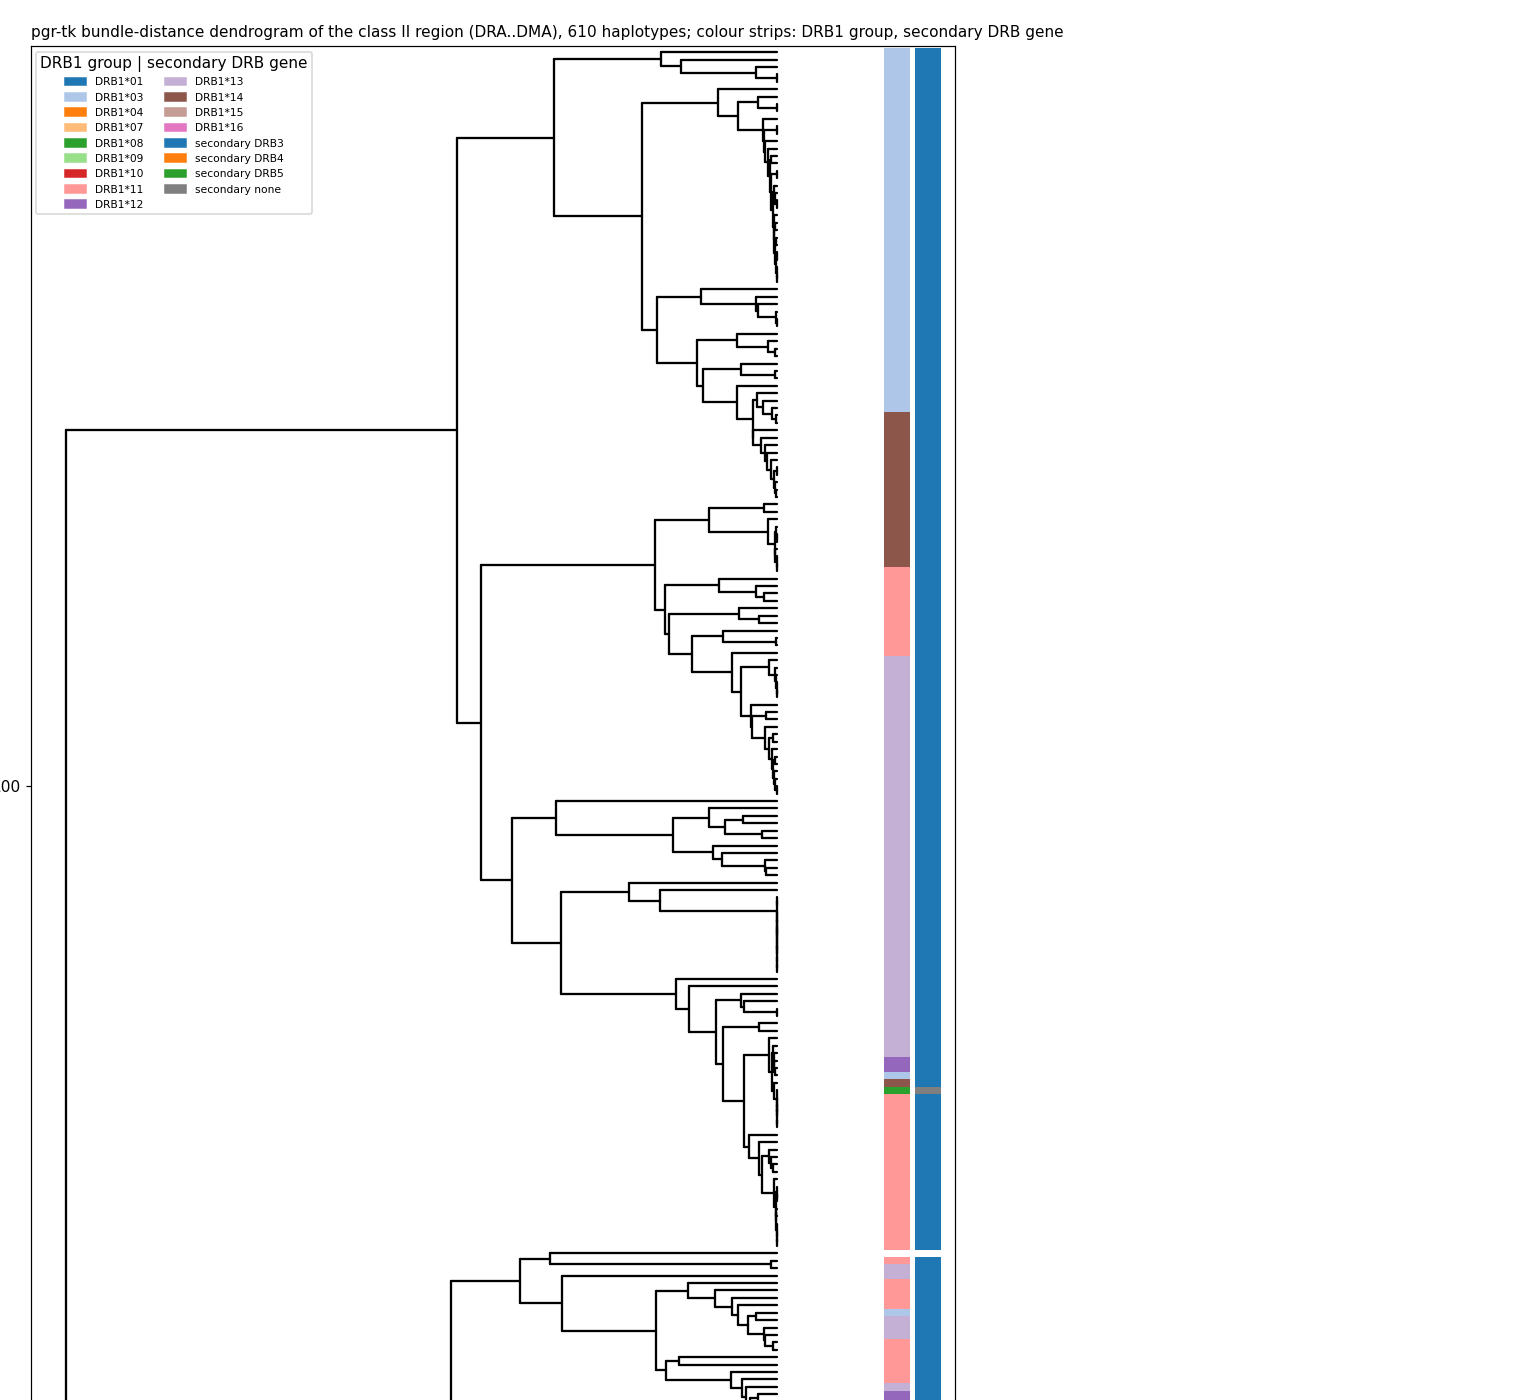
\includegraphics[height=0.78\textheight]{fig9_dendrogram_top.png}
  \src{Top of the pgr-tk bundle-distance dendrogram of 610 class II haplotypes; strips: DRB1 group, secondary DRB gene. Full tree: fig9\_classII\_dendrogram.png}
\end{frame}

\begin{frame}{The class II bundle graph is linear except for the DRB block}
  \centering
  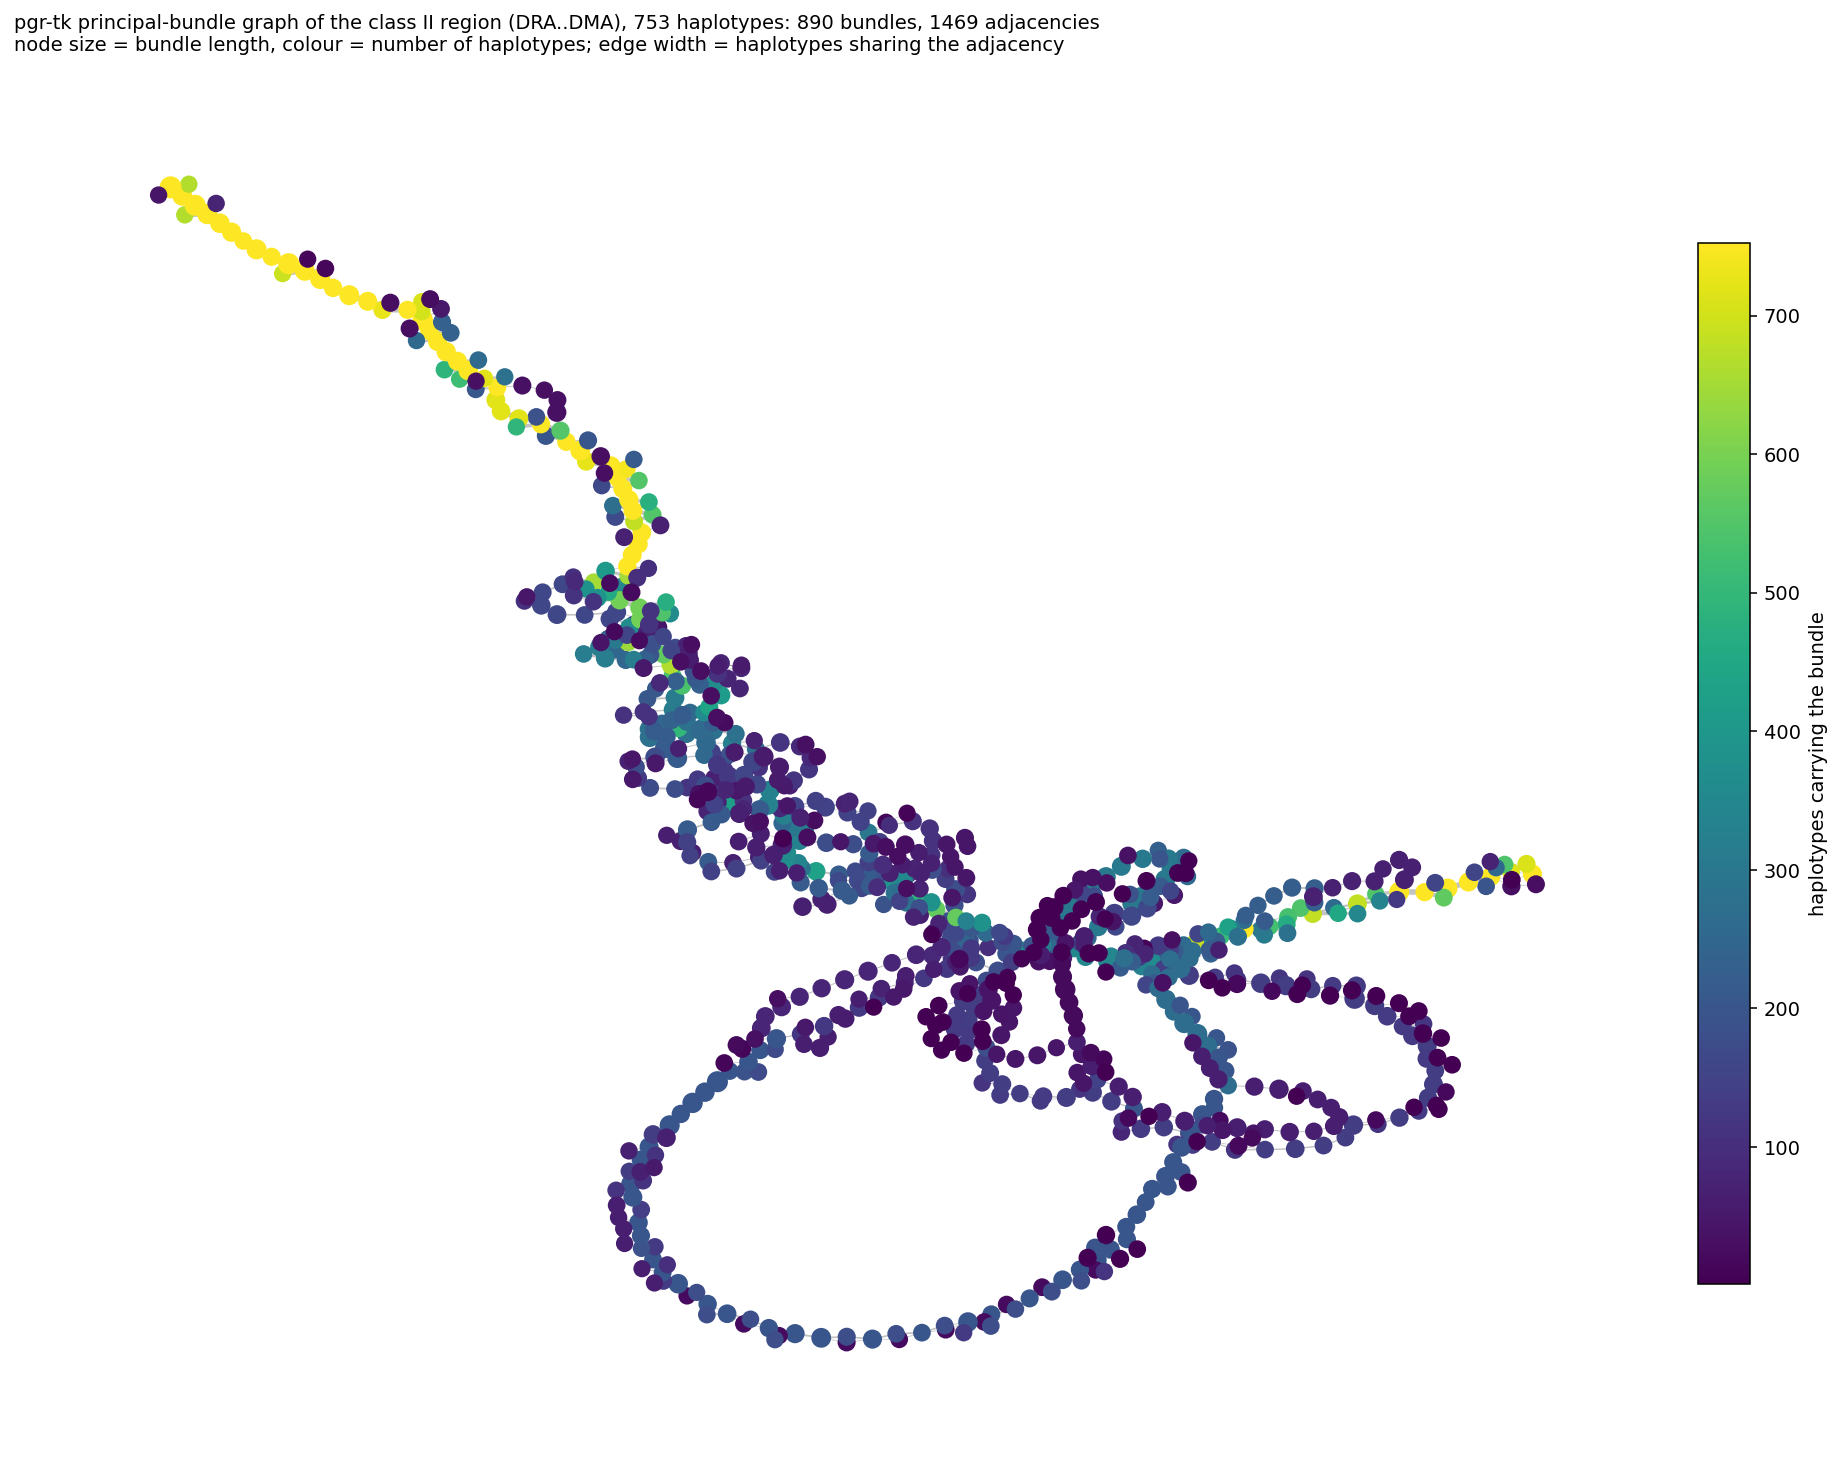
\includegraphics[height=0.78\textheight]{fig10_classII_bundle_graph.png}
  \src{863 principal bundles, node size = bundle length, colour = haplotypes carrying it, edges = consecutive bundles on a haplotype}
\end{frame}

\begin{frame}{Per-gene pangenome graphs for 19 HLA genes, all 610 haplotypes}
  \centering
  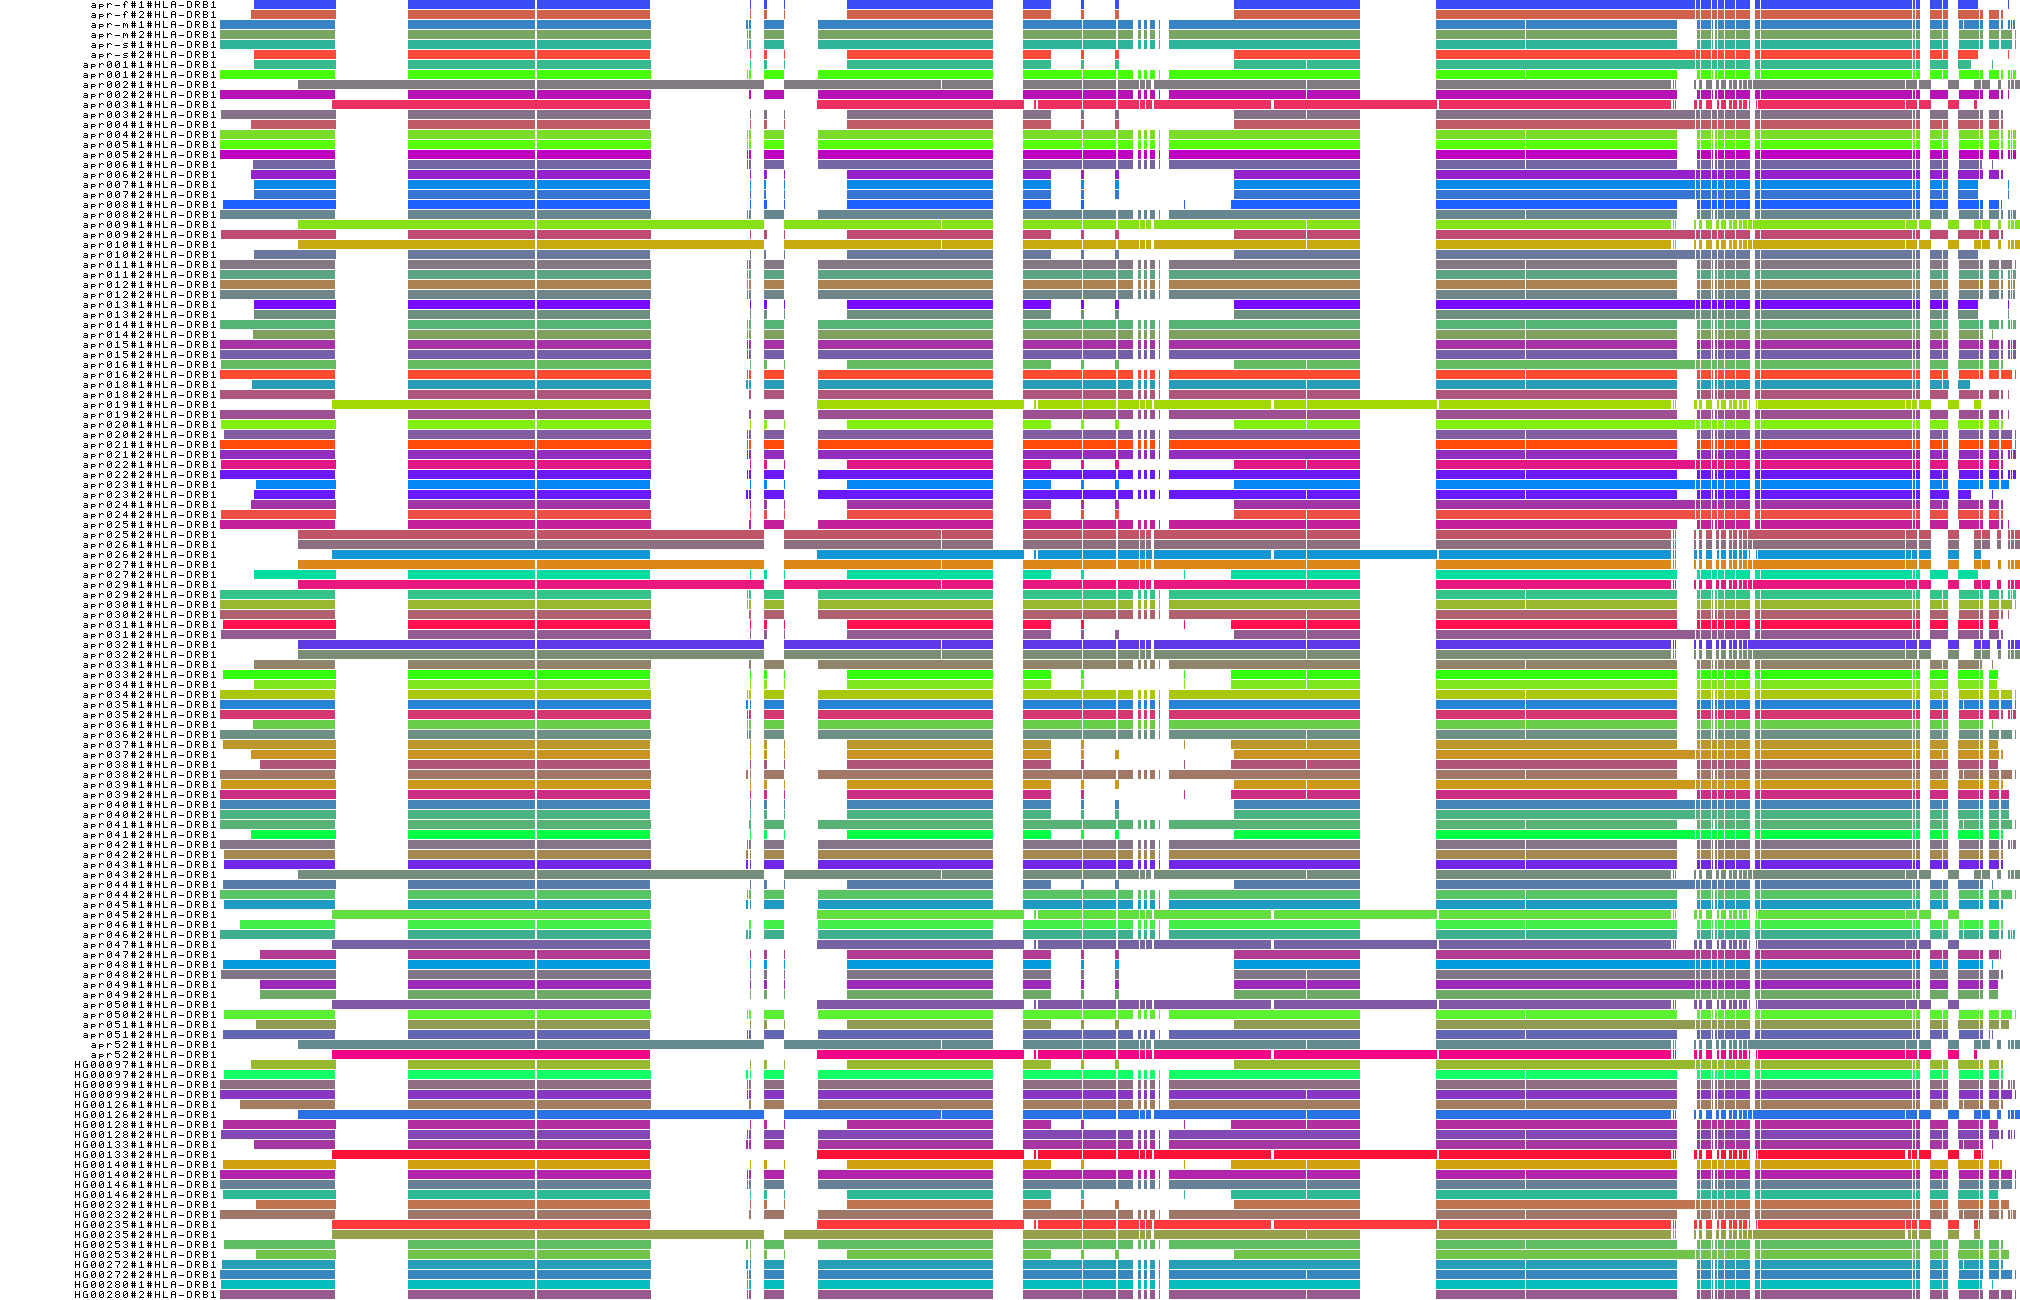
\includegraphics[height=0.64\textheight]{drb1_odgi_viz_top.png}
  \begin{itemize}
    \item HLA-DRB1 pggb graph (odgi viz, top rows of 610): rows are haplotypes, x is the graph, colour = path coverage
    \item Also per gene: pgr-tk bundle plot (SVG/HTML), dendrogram, MAP-graph GFA; whole-MHC bundle plot
  \end{itemize}
\end{frame}

\begin{frame}{Take-home}
  \begin{itemize}
    \item Assembly-based HLA typing across three pangenome projects reproduces known population frequencies and reveals data problems (duplicated haplotype, homozygous individuals) that short reads alone would not
    \item 60--78\% of DRB1 gene copies have no full-length match in IPD-IMGT/HLA; Arab haplotypes (APR + Saudi, 124) are a submission-ready resource once read support is added
    \item pgr-tk bundle decomposition recovers DR haplogroup structure without any allele calls; scales from 94 to 610 haplotypes
    \item Open: APR and JaSaPaGe raw reads for novel-allele validation; KIR and IGH with the same workflow; HPRC per-population split
    \item Workflow, scripts, figures and tables: \texttt{github.com/leechuck/pangenome-bh26} (\texttt{hla/})
  \end{itemize}
\end{frame}

\end{document}
